\section*{2.4 Mixture of trees with observable variables}

\begin{tcolorbox}
\textbf{Question 2.4.12:}
Implement this EM algorithm.
\end{tcolorbox}
Note: Due to the unclear instructions of point 4 in the EM-algorithm I discussed with Ludvig Doeser if the problem formulation meant that the node names should carry over to the new tree $T_k'$ or not.
\\

The EM algorithm was implemented as instructed using the provided Tree package and sieving was implemented in the following manner.

\begin{algorithm}[H]
\SetAlgoLined
\KwInput{Data samples}
\KwOutput{Tree mixture}

  Create a set of 100 Tree Mixtures $ \{ TM_i \}_{i=1}^100$

  For each Tree Mixture $TM_i$ do Expectation Maximisation for $10$ iterations

  Continue Expectation Maximisation for $90$ iterations on the $10$ Tree Mixtures with the highest likelihood

  Return the Tree Mixture with the highest likelihood as the inferred mixture

  \caption{EM algorithm with sieving}
\end{algorithm}

\begin{tcolorbox}
\textbf{Question 2.4.13:}
Apply your algorithm to the provided data and show how well you reconstruct the mixtures. First, compare the real and inferred trees with the unweighted Robinson-Foulds (aka symmetric difference) metric. Do the trees have similar structure? Then, compare the likelihoods of real and inferred mixtures.
\end{tcolorbox}
The following result was achieved when applying the EM-algorithm to the provided data.

\begin{figure}[H]
  \centering
  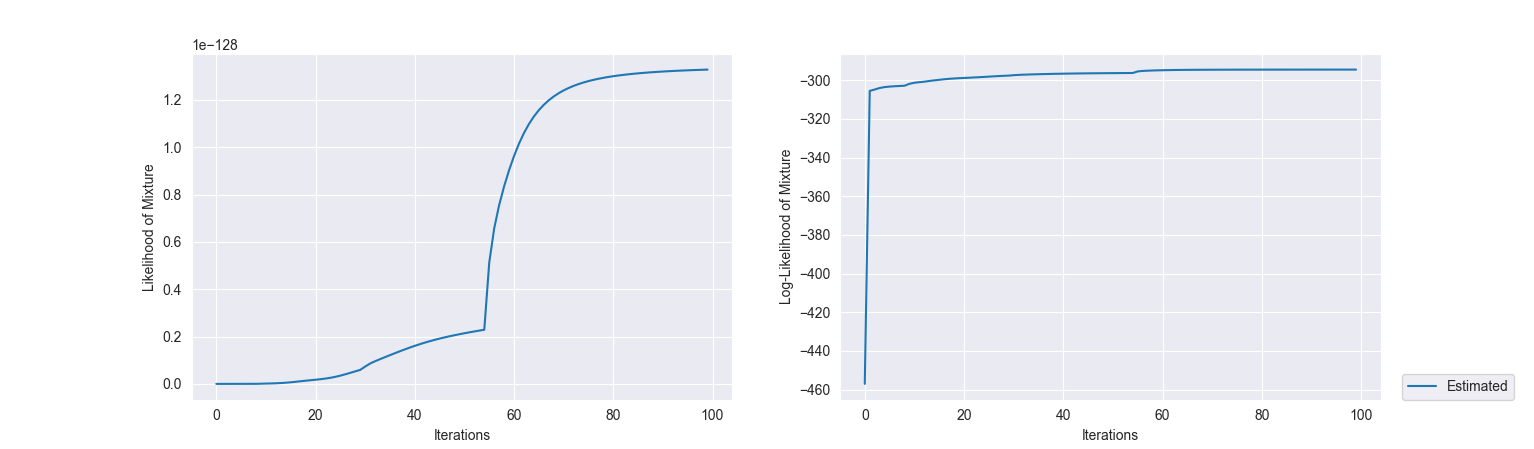
\includegraphics[width = \linewidth]{em_likelihoods.png}
  \caption{Convergence of EM}
  \label{EM_convergence}
\end{figure}

Judging by Figure \ref{EM_convergence} the likelihood is monotonically increasing which is a good indication that the EM-algorithm is working. The Robinson-Foulds metric was computed between the two mixtures which gave the following result.


\begin{table}

  \centering
  \begin{tabular}{ | c | c | c | c |}
  \hline
   & Inferred tree 0 & Inferred tree $1$ & Inferred tree $2$ \\ \hline
  Real tree $0$ & $4$ & $6$ & $4$ \\ \hline
  Real tree $1$ & $3$ & $5$ & $5$  \\ \hline
  Real tree $2$ & $4$ & $4$ & $4$  \\ \hline
  \end{tabular}
  \caption{RF-metric between real and inferred mixture}
  \label{RF-metric_real_inferred}
\end{table}

the trees had the following topology arrays

\begin{table}[H]

  \centering
  \begin{tabular}{ | c | c | c | c | c | c |}
  \hline
  Real tree $0$ & $nan$ & $0$ & $0$ & $1$ & $3$\\ \hline
  Real tree $1$ & $nan$ & $0$ & $0$ & $0$ & $3$  \\ \hline
  Real tree $2$ & $nan$ & $0$ & $0$ & $0$ & $0$  \\ \hline
  Inferred tree $0$ & $nan$ & $4$ & $0$ & $2$ & $3$ \\ \hline
  Inferred tree $1$ & $nan$ & $2$ & $0$ & $4$ & $2$  \\ \hline
  Inferred tree $2$ & $nan$ & $0$ & $0$ & $1$ & $2$  \\ \hline
  \end{tabular}
  \caption{Topology arrays of the different trees}
  \label{topology_array}
\end{table}

Judging by Tables \ref{RF-metric_real_inferred} and \ref{topology_array} the real trees and the inferred trees are not very similar in structure. The following likelihoods were obtained on the provided data.

\begin{table}[H]

  \centering
  \begin{tabular}{ | c | c |}
  \hline
  Mixture & LogLikelihood \\ \hline
  Real Mixture & $-311.4$\\ \hline
  Inferred Mixture & $-294.2$\\ \hline
  \end{tabular}
  \caption{LogLikelihoods of the mixtures}
  \label{Likelihood}
\end{table}

I believe that the inferred mixture achieves a higher loglikelihood due to being more specified on the $100$ provided samples than the real mixture and is thus overfitted to the data.

\begin{tcolorbox}
\textbf{Question 2.4.14:}
Simulate new tree mixtures with different number of nodes, samples and clusters. Try to find some interesting cases. Analyse your results as in the previous question.
\end{tcolorbox}

\textbf{Simulated tree mixture 1:}
The first tree mixture simulated from was made up of $2$ clusters having $10$ nodes each. $100$ samples was generated from the tree mixture and used to train the inferred mixture, this yielded the following results.

\begin{figure}[H]
  \centering
  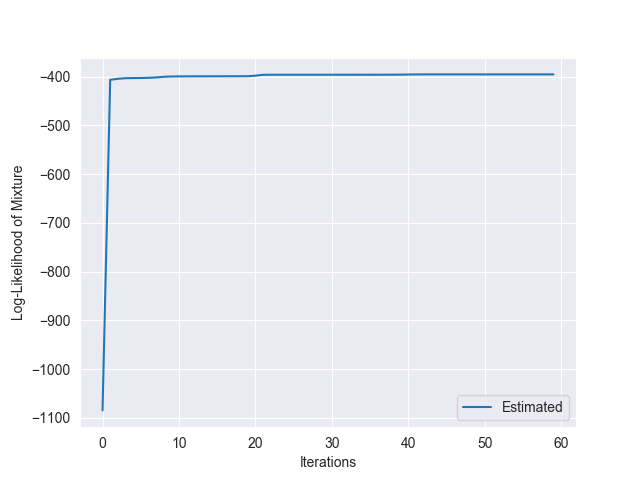
\includegraphics[width = \linewidth]{em_likelihoods_simulated_1.png}
  \caption{Convergence of EM simulated tree mixture 1}
  \label{EM_convergence_simulated_1}
\end{figure}

The likelihood was omitted from Figure \ref{EM_convergence_simulated_1} due to the low values.

\begin{table}

  \centering
  \begin{tabular}{ | c | c | c |}
  \hline
   & Inferred tree 0 & Inferred tree $1$ \\ \hline
  Simulated tree $0$ & $6$ & $10$ \\ \hline
  Simulated tree $1$ & $8$ & $10$ \\ \hline

  \end{tabular}
  \caption{RF-metric between simulated and inferred mixture}
  \label{RF-metric_simulated_1_inferred}
\end{table}

\begin{table}[H]

  \centering
  \begin{tabular}{ | c | c |}
  \hline
  Mixture & LogLikelihood \\ \hline
  Simulated Mixture $1$ & $-426.3$\\ \hline
  Inferred Mixture & $-395.6$\\ \hline
  \end{tabular}
  \caption{LogLikelihoods of the mixtures}
  \label{Likelihood_simulated_1}
\end{table}

The results are similar to the previous results both when it comes to the RF-metric and the loglikelihoods. The RF-metrics are about half of the maximum value of $20$ and the loglikelihood for the inferred mixture is greater than that of the simulated mixture.


\textbf{Simulated tree mixture 2:}
The second tree mixture simulated from was made up of $2$ clusters having $3$ nodes each. $10000$ samples was generated from the tree mixture and used to train the inferred mixture in order to see if the samples and inferred mixture will be more similar.

\begin{figure}[H]
  \centering
  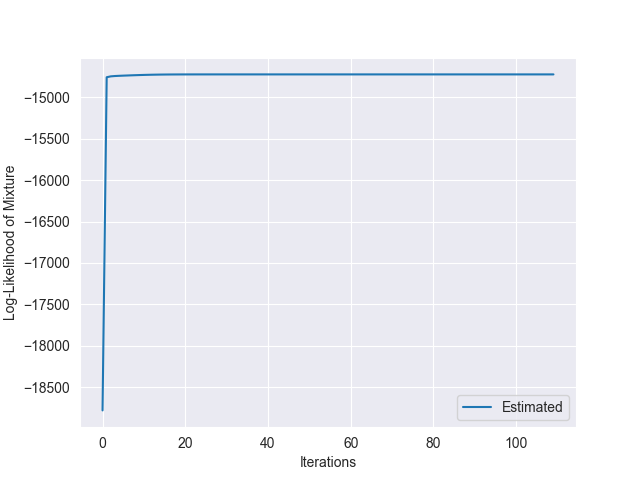
\includegraphics[width = \linewidth]{em_likelihoods_simulated_2.png}
  \caption{Convergence of EM simulated tree mixture 2}
  \label{EM_convergence_simulated_2}
\end{figure}

\begin{table}

  \centering
  \begin{tabular}{ | c | c | c |}
  \hline
   & Inferred tree 0 & Inferred tree $1$ \\ \hline
  Simulated tree $0$ & $0$ & $2$ \\ \hline
  Simulated tree $1$ & $2$ & $2$ \\ \hline

  \end{tabular}
  \caption{RF-metric between simulated and inferred mixture}
  \label{RF-metric_simulated_2_inferred}
\end{table}

\begin{table}[H]

  \centering
  \begin{tabular}{ | c | c |}
  \hline
  Mixture & LogLikelihood \\ \hline
  Simulated Mixture $2$ & $-14731.6$\\ \hline
  Inferred Mixture & $-14726.1$\\ \hline
  \end{tabular}
  \caption{LogLikelihoods of the mixtures}
  \label{Likelihood_simulated_1}
\end{table}

Again the results are similar as the loglikelihood for the inferred mixture is greater than the loglikelihood for the mixture sampled from. However in this example one of the inferred trees has the same structure as one of the trees that are simulated from. However it is unclear if this is just a coincidence due to the low number of nodes or if it is due to the increased number of training samples. If more time was given this could be further investigated.
